\documentclass[10pt,letter]{article}
\usepackage[utf8]{inputenc}
\usepackage{amsmath}
\usepackage{amsfonts}
\usepackage{amssymb}
\usepackage{graphicx}
\usepackage[margin=1in]{geometry}
\usepackage{float}


\begin{document}

\begin{titlepage}
\title{PHYS 5794 Homework 6}
\date{April 5, 2016}
\author{Thomas Edwards}
\maketitle
\end{titlepage}

\section{Problem 1}

\subsection{Problem Statement}
Write a code to evaluate the integral $\int_0^1 x^2 dx$, using a direct sampling in Monte Carlo method. The
direct sampling means using a uniform probability distribution function in your sampling. For this
problem, for simplicity, skip 100 initial sample points ($n_1 = 100$) and use the interval ($n_0 = 20$). The
algorithm for the direct sampling is the same as the importance sampling. Just the transition rate
is always unity and so the new configuration is always accepted. (15 pts)

\subsection{Method}

This problem was solved using the Monte Carlo method. In essence, the method works as follows:

\begin{itemize}
\item Select some random configuration $R_i$ within our domain $x \in [0,1).$
\item Use the random point to select a function evaluation $W(R_i).$
\item From the last configuration, find a new configuration such that $R_{i+1} = R_i + \Delta R$, where $\Delta R = \Delta(2\eta_i-1)$, and $\Delta$ is some chosen scaling factor.
\item Find and evaluate $P = W(R_{i+1})/W(R_{i})$.
\item Select a new random point $\zeta_i$  within our domain $x \in [0,1).$
\item If $\zeta_i \le P$ then accept the new configuration for $R_{i+1}$. Otherwise, set $R_{i+1}=R_i$.
\item Continue selecting new configurations from previous configurations, until the desired amount of configurations has been developed.
\end{itemize}

One you have your set of configurations, select a subset of them such that the configurations are not correlated. In this problem, we skipped the first 100 configurations, and began with $R_100$, and then continued by skipping every 20 configurations (for example, $R_{120}, R_{140},$ etc. )

We then evaluate our sum by finding the sample mean $\left\langle f \right\rangle = V\frac{1}{M}\sum_{i=0}^M f(R_i)$ where $M$ is the number of configurations used (not the number generated), $V$ is the volume of the configuration region (in this case 1), and $f(R_i)$ is the function we are trying to integrate evaluated with configuration $R_i$.

Further, we also calculate the standard deviation of the sample mean by finding 

$$ \sigma = V\sqrt{ \frac{\left\langle f^2 \right\rangle - \left\langle f \right\rangle^2}{M}},$$where $\left\langle f^2 \right\rangle = V\frac{1}{M}\sum_{i=0}^M f^2(R_i)$.

The values reported are in the form $\left\langle f \right\rangle \pm \sigma$.

\subsection{Verification of Program}

This program was verified by comparing it to the analytical value of the integral, which is $\frac{1}{3}$.

\subsection{Data}

The data from this program is below.

\begin{verbatim}
---------------
Number of Points:
10000
Numerical Integral:
0.338283705174 +/- 0.0134524717715
---------------
Number of Points:
20000
Numerical Integral:
0.32651383987 +/- 0.00924833087638
---------------
Number of Points:
30000
Numerical Integral:
0.335974603674 +/- 0.00777521333493
---------------
Number of Points:
40000
Numerical Integral:
0.32762110225 +/- 0.00662729163143
---------------
Number of Points:
50000
Numerical Integral:
0.342422438199 +/- 0.00601855212394
---------------
Number of Points:
60000
Numerical Integral:
0.337960787645 +/- 0.00542593128286
---------------
Number of Points:
70000
Numerical Integral:
0.340049162558 +/- 0.00502685520631
---------------
Number of Points:
80000
Numerical Integral:
0.331778899473 +/- 0.00466913946471
---------------
Number of Points:
90000
Numerical Integral:
0.330270469969 +/- 0.00440264389047
---------------
Number of Points:
100000
Numerical Integral:
0.329237976204 +/- 0.00418126266299
---------------
Number of Points:
110000
Numerical Integral:
0.327991162187 +/- 0.00395923878747
---------------
Number of Points:
120000
Numerical Integral:
0.33105274815 +/- 0.00384509101911
---------------
Number of Points:
130000
Numerical Integral:
0.331134544815 +/- 0.00367729070698
---------------
Number of Points:
140000
Numerical Integral:
0.334413062602 +/- 0.00355503196703
---------------
Number of Points:
150000
Numerical Integral:
0.329683650537 +/- 0.00341787712829
\end{verbatim}

\subsection{Analysis and Interpretation}

From the data above, we see that the integral is solved fairly well with the method implemented. The analytic result ($0.\bar{3}$) are more or less always within the standard deviation of the numerical results.

As the number of points is scaled, we see that the standard deviation also decreases with a scaleing of $1/\sqrt{M}$ as shown in the plot below.
\begin{figure}[H]
  \centering
    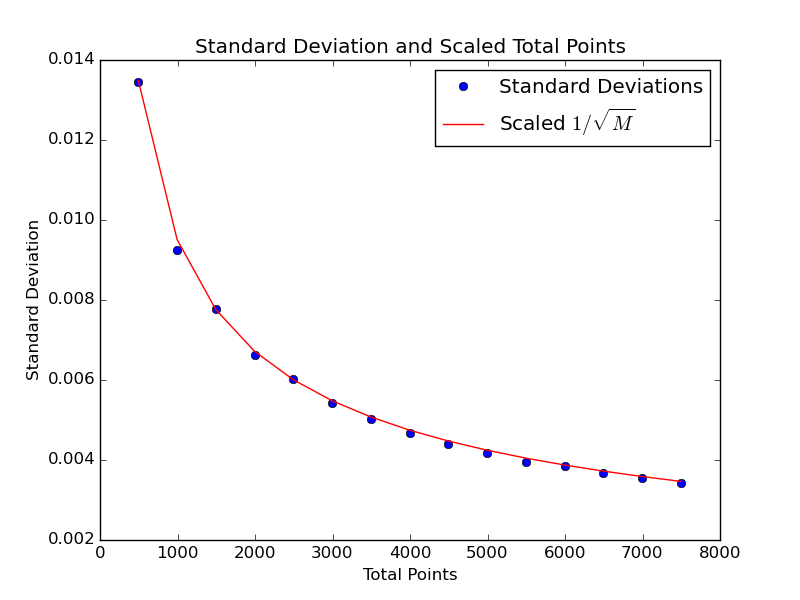
\includegraphics[width=.6\textwidth]{homework7_problem1_plot0}
\end{figure}

\subsection{Log}

This problem took approximately 3 hours.

\section{Problem 2}

This program was verified by comparing it to the analytical value of the integral, which is $\frac{1}{3}$.

\subsection{Problem Statement}

Write a code to evaluate the integral $\int_0^1 x^2 dx$, the standard deviation of the sample mean, and the autocorrelation
function (as a function of the number of Monte Carlo steps to be skipped, ($n_0 = l_c$), using
an importance sampling in Monte Carlo method. In the importance sampling, the following probability
distribution function can be used: $W(x) = C(x^2 + 10)$ where $C$ is a normalization constant that
needs to be determined. 

\subsection{Method}

The method for this problem is essentially identical to that of the first, but instead of using a $W(R_i)$ that is a uniform distribution, we instead use $W(x) = C(x^2 + 10)$. Since we require that the integral of $W$ over all space be 1, we can solve for $C$ by integrating $W(x)$ over our domain $x \in [0,1).$ Doing this gives us a normalization constant of approximately $0.0967741935484$, as shown in the data section.

In order to determine the number of points to skip, the autocorrelation function is determined and plotted serparately. This is done by finding

$$C(l) = \frac{\left\langle A_{n+l}A_{n} \right\rangle - \left\langle A_{n}\right\rangle^2  }{\left\langle A^2_{n}\right\rangle - \left\langle A_{n}\right\rangle^2} $$
where
$$ \left\langle A_{n+l}A_{n} \right\rangle = V\frac{1}{M}\sum_{i=0}^M A(R_{n+l}) A(R_{n}) $$
and
$$A(R_i) = \frac{f(R_i)}{W(R_i)}.$$

$C(l)$ was solved for a number of values of $l$, and the results of a sample run are shown below.

\begin{figure}[H]
  \centering
    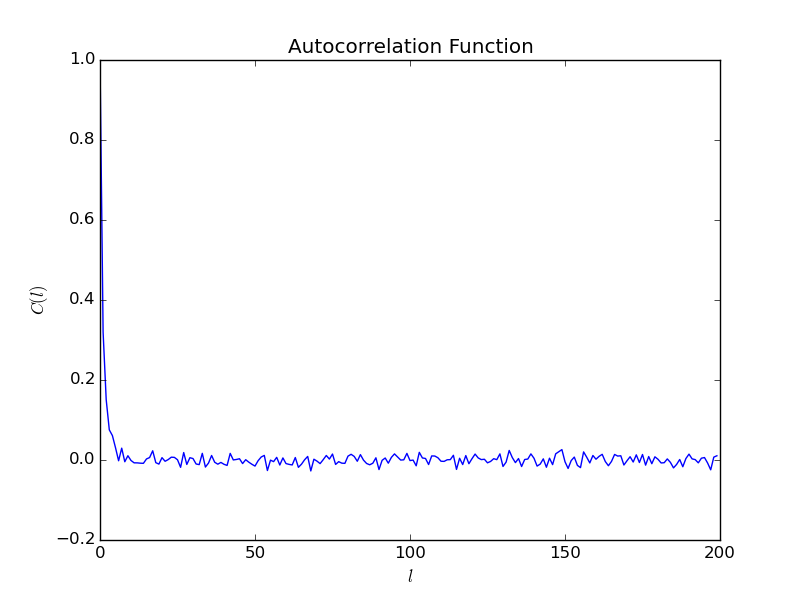
\includegraphics[width=.6\textwidth]{homework7_problem2_plot0}
\end{figure}

From here, we decide that $l=25$, just to give a significant amount of time for the values to anticorrelate.

\subsection{Verification of Program}

This program was verified by comparing it to the analytical value of the integral, which is $\frac{1}{3}$.

\subsection{Data}

The data for this section is below.

\begin{verbatim}Normalization Constant:
0.0967741935484
---------------
Number of Points:
10000
Numerical Integral:
0.350186693963 +/- 0.0139809949316
---------------
Number of Points:
20000
Numerical Integral:
0.327084093415 +/- 0.00971529642033
---------------
Number of Points:
30000
Numerical Integral:
0.343853445119 +/- 0.00824115465858
---------------
Number of Points:
40000
Numerical Integral:
0.332364326426 +/- 0.00708235889624
---------------
Number of Points:
50000
Numerical Integral:
0.325529767406 +/- 0.00629936458551
---------------
Number of Points:
60000
Numerical Integral:
0.335670402273 +/- 0.00593206986739
---------------
Number of Points:
70000
Numerical Integral:
0.331454277742 +/- 0.00532047778407
---------------
Number of Points:
80000
Numerical Integral:
0.335319793642 +/- 0.00512259438633
---------------
Number of Points:
90000
Numerical Integral:
0.33164729879 +/- 0.00471035880619
---------------
Number of Points:
100000
Numerical Integral:
0.337096836433 +/- 0.00453331609492
---------------
Number of Points:
110000
Numerical Integral:
0.328562317853 +/- 0.00433193262313
---------------
Number of Points:
120000
Numerical Integral:
0.328068846454 +/- 0.00413944754527
---------------
Number of Points:
130000
Numerical Integral:
0.331014797987 +/- 0.0039456008371
---------------
Number of Points:
140000
Numerical Integral:
0.334428375976 +/- 0.0038573383113
---------------
Number of Points:
150000
Numerical Integral:
0.334019240664 +/- 0.00373352303435
\end{verbatim}

\subsection{Analysis and Interpretation}

From the data above, we see that the integral is (again) solved fairly well with the method implemented. The analytic result ($0.\bar{3}$) are more or less always within the standard deviation of the numerical results, although it should be noted that this problem scaled the standard deviation much faster than the previous method.

As the number of points is scaled, we see that the standard deviation also decreases with a scaleing of $1/\sqrt{M}$ as shown in the plot below.
\begin{figure}[H]
  \centering
    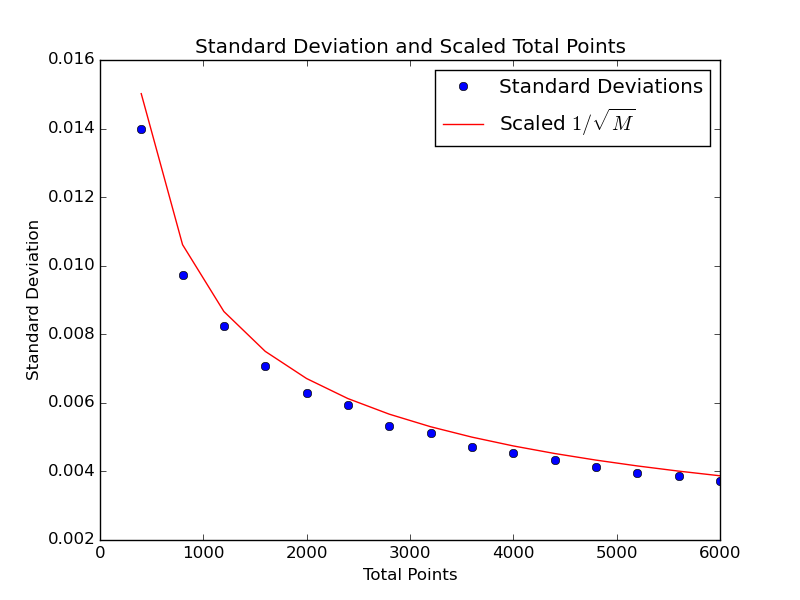
\includegraphics[width=.6\textwidth]{homework7_problem2_plot1}
\end{figure}

\subsection{Log}

The problem took approximately 6 hours.

\end{document}